\documentclass[a4paper,11pt]{article}

% Packages
\usepackage[margin=1in]{geometry}      % Page layout
\usepackage{titlesec}                  % Section formatting
\usepackage{enumitem}                  % Custom lists
\usepackage{fontawesome5}              % Icons
\usepackage{fancyhdr}                  % Header & Footer
\usepackage{graphicx}                  % For photo
\usepackage{hyperref}                  % Links
\usepackage{comment}
\usepackage{hyperref}
\usepackage{simpleicons}

\graphicspath{{swaraj-sodadasi-profile-photos/}}

% Font (ATS-friendly sans-serif)
\renewcommand{\familydefault}{\sfdefault}

% Section styling
\titleformat{\section}{\large\bfseries}{}{0em}{}[\titlerule]

% Footer for last updated
\fancyhf{}
\fancyfoot[L]{Last Updated: \today}
\pagestyle{fancy}

% Document starts
\begin{document}

% === Header with Name, Designation & Photo in one line ===
\begin{tabular*}{\textwidth}{@{}l@{\extracolsep{\fill}}r@{}}
    % Left side: Introduction details
    \begin{minipage}[t]{0.80\textwidth}
        \textbf{\LARGE Swaraj Sodadasi} \\[4pt]
        \textit{Computer Science Graduate and Aspiring Researcher} \\[8pt]
        \textbf{Email:} \href{mailto:swarajacc12004@gmail.com}{swaraj-sodadasi}
        \textbf{Linkedin:} \href{https://www.linkedin.com/in/swaraj-sodadasi-3b5362262/}{swaraj-sodadasi}
        \textbf{GitHub:} \href{https://github.com/swaraj-sodadasi}{swaraj-sodadasi}
        \textbf{Stack Overflow:} \href{https://stackoverflow.com/users/21460816/swaraj-sodadasi?tab=profile}{swaraj-sodadasi}
        \textbf{ORCID:} \href{https://orcid.org/0009-0008-7500-8038}{swaraj-sodadasi}
    \end{minipage}

     \begin{minipage}[t]{0.20\textwidth}
        \vspace{-10pt} % Pull photo slightly up
        \fbox{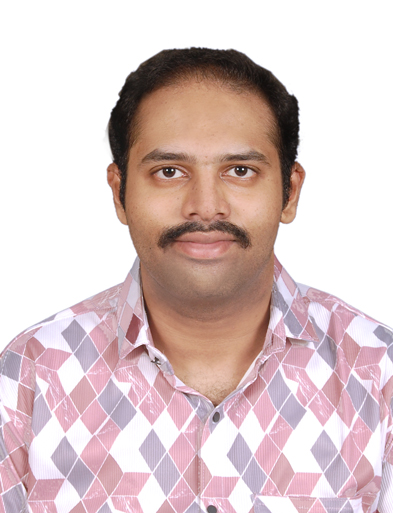
\includegraphics[width=2.5cm]{2025.jpg}}
     \end{minipage}

\end{tabular*}

% === Education Section ===
\section*{\textbf{Education}}
\begin{itemize}
	\item \textbf{Bachelor of Technology in Computer Science and Engineering} \hfill 2021--2025 \\
	\textit{Sri Vasavi Engineering College}, JNTUK, Andhra Pradesh \\
	CGPA: 8.96/10
\end{itemize}

% === Technical Skills Section ===
\section*{\textbf{Technical Skills}}
\begin{itemize}
    \item \textbf{Programming Languages:} C++ 23, Java SE, Bash, Python
    \item \textbf{Domain Knowledge (GATE-CS):} 
          Data Structures \& Algorithms, Operating Systems, Computer Organisation \& Architecture,
          Computer Networks, Database and Management Systems, Theory of Computation,
          Compiler Design
    \item \textbf{Database Management Systems:} PostgreSQL, MongoDB
    \item \textbf{Web Frameworks:} Jakarta EE, FastAPI, ReactJS
    \item \textbf{Cloud Technology:} Microsoft Azure
    \item \textbf{Machine Learning:} TensorFlow, PyTorch
    \item \textbf{Tools \& Platforms:} Docker, IDE's, LATEX, Office Productivity
    \item \textbf{Application Software:} AutoCAD
\end{itemize}

% === Projects Section ===
\section*{\textbf{Projects}}
\begin{itemize}[leftmargin=*]

   \item \textbf{Weather Assistant}  \\
    	  \textbf{Role} Lead Developer	\\
          \textbf{Description} In this system a user can get the weather information of a location using voice command. \\
          \textbf{Technologies: JavaScript, REST API, Microsoft Azure}

    \item \textbf{MedIntel (Converging CNN-Powered Deep Learning and Healthcare Informatics: A TensorFlow-Based Framework for Medical Image Analysis and Scalable Patient Data Management)}  \\
    	  \textbf{Role} Lead Developer	\\
          \textbf{Description} This system focuses to analyze medical images for the detection of abnormalities with addition to that we will be having a fully functional and scalable patient management system. \\
          \textbf{Technologies: Python, FastAPI, PostgreSQL, TensorFlow, Deep Learning}

    \item \textbf{A Real-Time Graph-Driven Lightweight Adaptive and Application-Aware IDS for Linux Based Personal Networks}  \\
    	  \textbf{Role} Independent System Developer	\\
          \textbf{Description} This system will monitor the network signals for detecting intrusions and it will predict the attacks based on custom made model with periodic alerts and notifications. \\
          \textbf{Technologies: JavaFX, Pytorch, Boost library, PostgreSQL, Fedora Linux, Grafana, Prometheus, AppImage}
          
\end{itemize}


\section{\textbf{Publications} {\scriptsize C=Conference, J=Journal, P=Patent, S=In Submission, T=Thesis}}
\vspace{0.2mm}
\small{
\begin{enumerate}[leftmargin=*, labelsep=0.5em, align=left, widest={[\textbf{S.1}]}, itemindent=0em, label={\textbf{[\arabic*]}]}]
\item[\textbf{[J.1]}] Swaraj Sodadasi, Prasanthi, Srinivasan, Shyam, Kumar, Nagesh, Pujan. \\
\href{https://rjpn.org/jetnr/viewpaperforall.php?paper=JETNR2503029}{\textbf{Converging CNN-Powered Deep Learning and Healthcare Informatics: A TensorFlow-Based Framework for Medical Image Analysis and Scalable Patient Data Management}}. \\
\textit{JETNR - JOURNAL OF EMERGING TRENDS AND NOVEL RESEARCH (www.JETNR.org)}, ISSN:2984-9276, Vol.3, Issue 3, page no.a266-a276, March-2025
\end{enumerate}
}


% === Certifications Section ===
\section*{\textbf{Certifications}}

\begin{itemize}[leftmargin=*]

    \item \textbf{}
    \begin{itemize}
        \item Issued by: Amazon Web Services (AWS)
        \item Credential URL: \href{https://www.credly.com/users/sodadasi-swaraj}{swaraj-sodadasi}
    \end{itemize}

\end{itemize}


% Competitive Programming Profiles Section
\section*{\textbf{Competitive Programming Profiles}}
\begin{itemize}
    \item \href{https://www.hackerrank.com/profile/swarajacc12004} {\textbf{HackerRank}}
    \item \href{https://auth.geeksforgeeks.org/user/geeksforgeeksacc1} {\textbf{GeeksforGeeks}}
\end{itemize}


% === Languages Section ===
\section*{\textbf{Languages}}
\begin{itemize}[leftmargin=*]
    \item \textbf{English:} Professional Working Proficiency
    \item \textbf{Telugu:} Native Proficiency
    \item \textbf{Hindi:} Conversational Proficiency
    \item \textbf{Japanese:} Basic Proficiency
\end{itemize}


\section*{\textbf{Professional Achievements and Other Activities}}
\begin{itemize}[leftmargin=*]
    \item Qualified GATE 2026 in Computer Science and Information Technology
    \item An active member of "chess.com" utilising chess for patience and strategic decision making skills
\end{itemize}

\end{document}

